\documentclass[11pt,a4paper]{article}
\usepackage{fontspec}
\setmainfont{Noto Serif}
\setsansfont{Noto Sans}
\usepackage[french]{babel}
\usepackage[a4paper,top=2.25cm,bottom=2.25cm,left=2.55cm,right=2.55cm]{geometry}
\usepackage{microtype}
\usepackage{amsmath,amssymb}
\usepackage{booktabs,tabularx,longtable,array,multirow}
\usepackage{graphicx}
\usepackage{caption}
\usepackage[table]{xcolor}
\usepackage{enumitem}
\usepackage{titlesec}
\usepackage{fancyhdr}
\usepackage{lastpage}
\usepackage{hyperref}
\usepackage{float}
\usepackage{needspace}
\usepackage{setspace}
\usepackage{ragged2e}
\definecolor{navy}{HTML}{192E49}
\definecolor{blue}{HTML}{0A6A91}
\definecolor{amber}{HTML}{B16A1E}
\definecolor{pale}{HTML}{F2F6F9}
\definecolor{line}{HTML}{D4DFE6}
\definecolor{graytext}{HTML}{526579}
\hypersetup{colorlinks=true,linkcolor=navy,urlcolor=blue,citecolor=blue,pdftitle={Google Trends : critique methodologique et journal des experiences},pdfauthor={Projet Math Finance}}
\setlength{\parindent}{0pt}
\setlength{\parskip}{5.2pt}
\setlength{\emergencystretch}{1.8em}
\setlist[itemize]{topsep=2pt,itemsep=2pt,leftmargin=1.4em}
\setlist[enumerate]{topsep=2pt,itemsep=3pt,leftmargin=1.5em}
\titleformat{\section}{\Large\bfseries\sffamily\color{navy}}{\thesection}{0.7em}{}
\titleformat{\subsection}{\large\bfseries\sffamily\color{blue}}{\thesubsection}{0.65em}{}
\titleformat{\subsubsection}{\normalsize\bfseries\sffamily\color{navy}}{\thesubsubsection}{0.65em}{}
\titlespacing*{\section}{0pt}{16pt}{6pt}
\titlespacing*{\subsection}{0pt}{10pt}{4pt}
\captionsetup{font=small,labelfont={bf,color=navy},skip=6pt}
\renewcommand{\arraystretch}{1.16}
\pagestyle{fancy}
\fancyhf{}
\fancyhead[L]{\small\sffamily\textcolor{graytext}{PROJET MATH FINANCE / NOTE MÉTHODOLOGIQUE}}
\fancyhead[R]{}
\fancyfoot[L]{\footnotesize\textcolor{graytext}{Réplication de Salisu \& Badmus (2026)}}
\fancyfoot[R]{\footnotesize\textcolor{graytext}{Page \thepage/\pageref{LastPage}}}
\renewcommand{\headrulewidth}{0.35pt}
\renewcommand{\footrulewidth}{0pt}
\setlength{\headheight}{16pt}
\newcommand{\source}[1]{\par\vspace{-2pt}{\footnotesize\color{graytext}\textit{Source :} #1}\par}
\newcommand{\keybox}[2]{\vspace{5pt}\noindent\colorbox{pale}{\parbox{\dimexpr\linewidth-2\fboxsep\relax}{\vspace{5pt}\textbf{\color{navy}#1}\par #2\vspace{5pt}}}\vspace{5pt}}
\newcommand{\pct}{\,\%}
\newcolumntype{Y}{>{\RaggedRight\arraybackslash}X}
\newcolumntype{Z}{>{\RaggedLeft\arraybackslash}X}
\begin{document}
\begin{titlepage}
\thispagestyle{empty}
\vspace*{1.2cm}
{\sffamily\color{blue}\large ÉTUDE DE RÉPLICATION ÉCONOMÉTRIQUE \hfill NOTE DE RECHERCHE}\par
\vspace{0.7cm}
{\color{navy}\rule{\textwidth}{1.3pt}}\par
\vspace{1.25cm}
{\sffamily\fontsize{26}{31}\selectfont\bfseries\color{navy} Google Trends :\\ critiques méthodologiques,\\ expériences de collecte et\\ décision de reproduction}\par
\vspace{0.65cm}
{\large\color{graytext} Application à la prévision des primes de risque et de la volatilité du marché boursier américain}\par
\vspace{1.0cm}
\keybox{Décision de l'équipe}{Conserver, pour la réplication principale, les deux séries mensuelles originales du terme de recherche «\,Artificial Intelligence\,» : \textbf{Google Web Search} et \textbf{Google News Search}, monde entier, toutes catégories, janvier 2012 -- décembre 2024. Les expériences alternatives restent documentées mais ne remplacent pas ces séries.}
\vfill
\begin{tabularx}{\textwidth}{@{}>{\bfseries\color{navy}}lY@{}}
Étude de référence & Salisu, A. A. et Badmus, S. (2026), \emph{Can AI News Improve the Out-of-Sample Forecasts of Risk Premia and Volatility in the U.S. Stock Market?}, \emph{Quality \& Quantity}.\\
Équipe & Aziz Gharbi et Selima Bellil\\
Cadre & Projet Math Finance — documentation de la collecte, semaine 3\\
État & Séries retenues, divergences documentées, reproduction numérique non exacte\\
\end{tabularx}
\vspace{0.5cm}
{\color{navy}\rule{\textwidth}{1.3pt}}\par
\end{titlepage}
\tableofcontents
\clearpage

\section{Synthèse et choix méthodologique}
\textbf{Objet.} Ce document rassemble les contrôles de qualité et les expériences réalisés pour comprendre les écarts entre les séries Google Trends collectées par notre équipe et celles publiées par Salisu et Badmus (2026) \cite{SalisuBadmus2026}. Il fixe un protocole reproductible pour la suite des estimations, sans modifier artificiellement les valeurs téléchargées.

Les séries \emph{AI News Search} et \emph{AI Web Search} du rapport sont des \textbf{indices d'intérêt de recherche} entre 0 et 100. Elles ne sont ni des volumes absolus de requêtes, ni des nombres d'articles publiés, ni des mesures automatiques de sentiment ou de pertinence économique \cite{GoogleFAQ,GoogleTerms}.

\begin{table}[H]
\centering\small
\caption{Périmètre définitif des séries principales}
\begin{tabularx}{\textwidth}{@{}lYY@{}}\toprule
Paramètre & AI News Search & AI Web Search\\\midrule
Expression & \multicolumn{2}{c}{\texttt{Artificial Intelligence} (terme de recherche)}\\
Périmètre géographique & \multicolumn{2}{c}{Monde entier (\texttt{geo=} vide)}\\
Catégorie & \multicolumn{2}{c}{Toutes catégories (\texttt{cat=0})}\\
Propriété Google & Google Actualités (\texttt{gprop=news}) & Recherche sur le Web (\texttt{gprop=} vide)\\
Période & \multicolumn{2}{c}{Janvier 2012 -- décembre 2024}\\
Granularité & \multicolumn{2}{c}{Mensuelle, 156 observations par série}\\
Traitement & Aucun recalibrage; tri et validation des dates & Aucun recalibrage; tri et validation des dates\\\bottomrule
\end{tabularx}
\end{table}

\keybox{Principe de fidélité à la source}{L'article mentionne explicitement la recherche «\,Artificial Intelligence\,» sur Google Trends Explore. La notation parfois plus large («\,AI\,» ou «\,Artificial Intelligence\,») utilisée plus loin crée une ambiguïté, mais ne justifie pas de choisir le terme qui rapproche le plus les moyennes. Le \textbf{terme complet} est conservé comme référence; \texttt{AI} reste une \textbf{analyse de sensibilité}.}

\section{Source et portée des variables de l'article}
Dans la section 2 de leur article, les auteurs déclarent avoir collecté des séries mondiales de recherches liées à l'IA depuis \href{https://trends.google.com/trends/explore}{Google Trends Explore}, avec une fréquence mensuelle et la période d'étude 2012--2024 \cite{SalisuBadmus2026}. La section 4.1 emploie aussi la formulation «\,AI\,» ou «\,Artificial Intelligence\,», sans donner un identifiant de requête complet ni un fichier original de séries brutes.

L'étude applique ces indicateurs à la prédiction des primes de risque et de la volatilité des actions américaines. La portée géographique des \emph{recherches} déclarée dans l'article est \textbf{mondiale}, indépendamment du fait que le marché étudié soit américain. Cette distinction a motivé notre contrôle d'une extraction limitée aux États-Unis, qui ne s'est pas révélée plus proche des statistiques publiées.

La \textbf{Table 1} de l'article donne \textbf{16,717} (écart-type \textbf{22,201}) pour \emph{AI News Search} et \textbf{14,904} (écart-type \textbf{20,214}) pour \emph{AI Web Search}. Les auteurs évoquent notamment \textbf{2} en janvier 2012 et \textbf{86} en mai 2024 pour les nouvelles IA. Ces points serviront de repères descriptifs, et non d'objectifs de calibrage \cite{SalisuBadmus2026}.

\section{Google Trends : mesure et critiques}
\subsection{Normalisation native : ce que signifie un indice entre 0 et 100}
Google Trends utilise des échantillons de recherches, agrégés et rapportés à la totalité des recherches dans le périmètre choisi. L'indice est ensuite mis à l'échelle sur la fenêtre temporelle et géographique demandée \cite{GoogleFAQ}. Pour une requête isolée, on peut représenter \emph{conceptuellement} cette procédure par
\[
 r_{q,t}=\frac{\text{volume échantillonné associé à }q\text{ au mois }t}
 {\text{volume total échantillonné de recherches au mois }t},
 \qquad
 GT_{q,t}\approx 100\frac{r_{q,t}}{\max_{s\in T}r_{q,s}}.
\]
Cette écriture simplifie les traitements internes non publics de Google; elle ne constitue pas une spécification complète de l'algorithme. \textbf{Le score 100 représente un maximum relatif pour la requête configurée}, et non un nombre déterminé de recherches.

La conséquence est essentielle : les deux séries Web et News extraites séparément possèdent chacune leur propre échelle relative 0--100. On peut étudier leur dynamique et leurs corrélations, mais il serait incorrect de conclure, par exemple, que «\,37,7 recherches Web\,» dépassent «\,26,5 recherches News\,» en volumes absolus.

\subsection{Cinq limites documentées}
\begin{enumerate}
\item \textbf{Échantillonnage et instabilité.} Deux téléchargements de paramètres identiques peuvent différer selon les échantillons et le moment de collecte; le mécanisme a été étudié notamment par Cebrián et Domenech \cite{Cebrian2024}.
\item \textbf{Normalisation conditionnelle.} La fenêtre, la région, les mots-clés comparés et le type de recherche influencent les valeurs affichées. Les exports indépendants ne forment pas automatiquement une échelle commune \cite{GoogleFAQ,GoogleTerms}.
\item \textbf{Terme littéral contre sujet.} Le \emph{terme de recherche} «\,Artificial Intelligence\,» ne recouvre pas nécessairement les autres langues et synonymes; le \emph{sujet} Google agrège davantage de formulations et peut construire une série différente \cite{GoogleTerms}.
\item \textbf{Seuils, arrondis et bruit.} Des requêtes peu fréquentes peuvent apparaître comme \texttt{0} ou \texttt{<1}; Google documente aussi un bruit statistique susceptible de produire des pics isolés \cite{GoogleFAQ}.
\item \textbf{Validité de construit.} L'intérêt pour une requête ne mesure directement ni le nombre d'articles, ni le signe d'une nouvelle, ni son effet financier. Une revue systématique de 360 études identifie des faiblesses récurrentes de validation et de fiabilité \cite{Misuse2025}.
\end{enumerate}

\subsection{Changements de méthode et millésimes de données}
Des travaux ont documenté des erreurs de mesure associées à l'évolution des procédés de collecte de Google Trends \cite{Liu2024}; d'autres observent des difficultés de comparaison autour du changement signalé en janvier 2022 pour \textit{Google Health Trends API} \cite{Health2022}. Toutefois, ces travaux \textbf{n'établissent pas} que notre écart numérique avec Salisu et Badmus découle précisément d'un changement de l'outil \emph{Explore} en 2025 ou 2026.

Google a annoncé en juillet 2025 une \emph{API officielle alpha} avec données à échelle stable entre requêtes et historique glissant d'environ cinq ans. Cette API ne correspond pas nécessairement à la normalisation de l'interface Explorer et ne donne pas, à elle seule, l'ensemble 2012--2024 \cite{GoogleAPI2025}. À l'inverse, la bibliothèque \texttt{pytrends} est un outil \textbf{non officiel}, et non une source indépendante conservant de vieux millésimes.

\section{Corpus définitivement retenu}
Les deux séries ont été retranscrites sans changement des valeurs à partir des exports communiqués à l'équipe; les \textbf{156 mois de janvier 2012 à décembre 2024} sont présents une seule fois. L'annexe \ref{annexe_donnees} restitue l'intégralité des 312 indices.

\begin{table}[H]
\centering\small
\caption{Statistiques descriptives vérifiées des séries retenues}
\begin{tabular}{@{}lrr@{}}\toprule
Caractéristique & AI News Search & AI Web Search\\\midrule
Nombre d'observations & 156 & 156\\
Valeurs manquantes & 0 & 0\\
Moyenne & 26,474 & 37,654\\
Écart-type empirique ($n-1$) & 18,997 & 22,014\\
Minimum & 4 & 11\\
Médiane & 25 & 38\\
Maximum & 100 & 100\\
Mois du maximum & juillet 2024 & mai 2023\\
\bottomrule\end{tabular}
\end{table}
La corrélation de Pearson entre les deux séries est \textbf{0,854} (arrondi à trois décimales). Cette association décrit la covariation temporelle des indices; elle n'implique ni causalité, ni égalité des volumes de recherche.

\begin{figure}[H]
\centering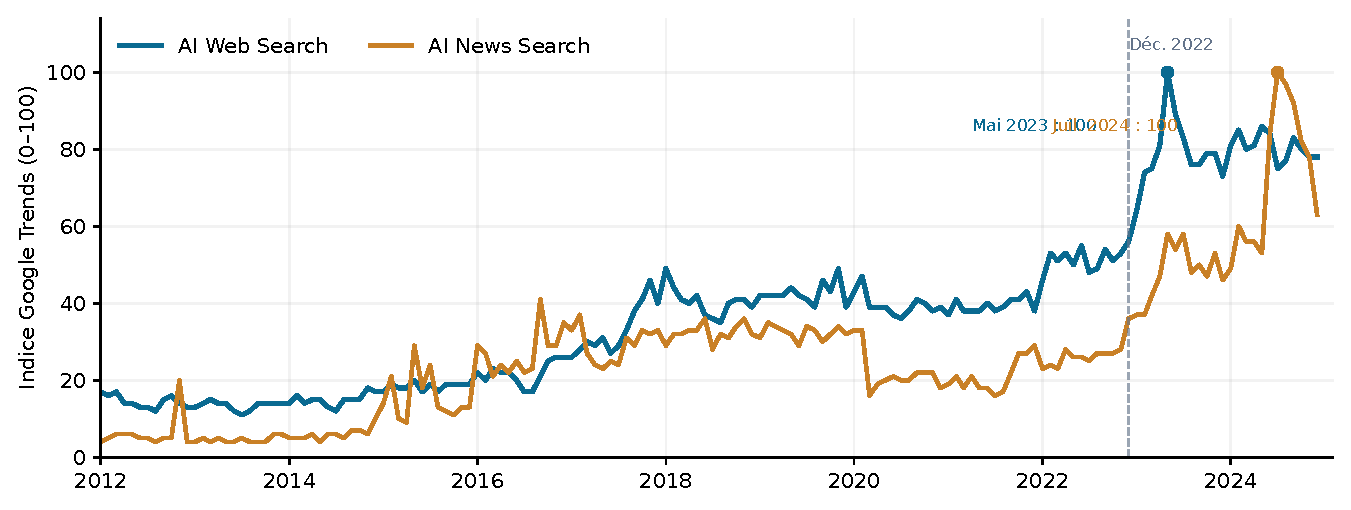
\includegraphics[width=\textwidth]{fig_series.pdf}
\caption{Évolution mensuelle des séries Google Trends conservées, 2012--2024. Chaque courbe dispose de sa propre normalisation issue d'une extraction distincte.}
\end{figure}

\begin{figure}[H]
\centering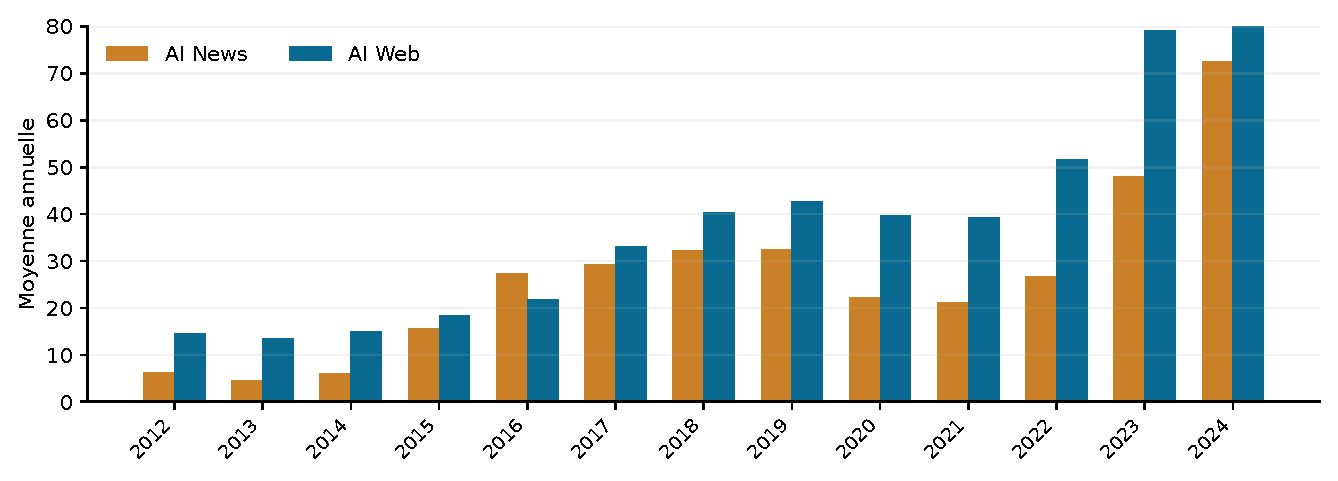
\includegraphics[width=0.98\textwidth]{fig_annees.pdf}
\caption{Moyennes annuelles : visualisation descriptive, non comparaison de volumes absolus.}
\end{figure}

\paragraph{Contrôle d'anomalies.} La valeur \textbf{20} du mois de novembre 2012 dans \emph{AI News Search} est élevée relativement à ses voisines (octobre : 5; décembre : 4). Elle doit être \textbf{signalée et conservée}, sauf preuve documentée d'une erreur d'extraction. L'effacer sans contrôle créerait une correction opportuniste.

\section{Journal des expériences de Google Trends}
Toutes les expériences ont été réalisées pour analyser les écarts avec l'article; elles \textbf{ne sont pas fusionnées} dans les indicateurs définitifs. Les chiffres ci-dessous viennent des fichiers d'export et des résultats de scripts de comparaison conservés au cours du projet. Le fichier CSV seul n'indique pas toujours la propriété Web/Actualités : les attributions suivent les réglages et URL confirmés au moment des expériences.

\begin{table}[H]
\centering\scriptsize
\caption{Expériences de collecte et principaux résultats}
\begin{tabularx}{\textwidth}{@{}>{\RaggedRight\arraybackslash}p{2.0cm}Yrr>{\RaggedRight\arraybackslash}p{2.4cm}@{}}\toprule
Expérience & Paramètres testés (par rapport à la série de base) & Moyenne & Éc.-type & Lecture\\\midrule
Web principal & Expression complète; monde; Web; 2012--2024 & 37,654 & 22,014 & Référence retenue\\
News principal & Expression complète; monde; News; 2012--2024 & 26,474 & 18,997 & Référence retenue\\
Web, «\,AI\,» & Mot bref \texttt{AI}; monde; Web & 21,385 & 21,922 & Alternative de requête\\
News, «\,AI\,» & Mot bref \texttt{AI}; monde; News & 19,917 & 24,954 & Alternative de requête\\
Web, États-Unis & Expression complète; \texttt{geo=US} & 37,814 & 19,703 & Effet géographique faible\\
Web, 2004--2024 & Expression complète; monde; données filtrées ensuite à 2012--2024 & 37,635 & 22,009 & Effet fenêtre faible\\
Web, É.-U. 2004--2024 & Expression complète; États-Unis; données filtrées à 2012--2024 & 37,814 & 19,703 & Effet fenêtre faible\\
Web, \texttt{pytrends} & Même expression et mêmes paramètres que Web principal & 37,635 & 22,009 & Cohérence avec CSV manuel\\
News, \texttt{pytrends} & Même expression et mêmes paramètres que News principal & 26,474 & 18,997 & Cohérence avec CSV manuel\\\bottomrule
\end{tabularx}
\end{table}

\subsection{Comparaison simultanée des deux mots-clés}
Deux exports comparaient \texttt{AI} et \texttt{Artificial Intelligence} sur une \textbf{échelle commune}, une fois sur Web et une fois sur News. Sur le Web, la série \texttt{AI} avait une moyenne \textbf{21,378}, contre \textbf{19,917} pour News. L'expression complète présentait une faible échelle dans ces comparaisons, avec des valeurs \texttt{<1} : il ne serait pas rigoureux de remplacer celles-ci arbitrairement par zéro puis de publier une moyenne exacte.

Dans l'expérience News, les 156 valeurs de \texttt{AI} téléchargées seules étaient identiques à celles de \texttt{AI} dans la comparaison à deux mots-clés. Cela \textbf{ne démontre pas} que l'ajout d'un terme ne modifie jamais la normalisation; dans notre cas, il n'a pas modifié cette colonne.

Le fichier d'un projet antérieur, \texttt{Technology\_\_AI.csv}, contient par ailleurs 241 observations \emph{quotidiennes} entre juillet 2025 et mars 2026 pour \emph{artificial intelligence}, \emph{machine learning}, \emph{generative ai} et \emph{ai tool}. Il illustre une approche multi-mots-clés mais \textbf{ne fournit pas} une série de 2012--2024 utilisable pour la réplication.

\subsection{Autres hypothèses discutées}
\begin{itemize}
\item \textbf{Majuscules/minuscules :} vérification écartée comme explication pertinente; aucun effet systématique reproduisant l'article.
\item \textbf{États-Unis plutôt que monde :} non soutenu pour la série Web; le pays de l'étude boursière ne détermine pas automatiquement la géographie des requêtes.
\item \textbf{Fenêtre 2004--2024 :} différence négligeable pour Web après restriction à 2012--2024.
\item \textbf{Interface contre \texttt{pytrends} :} résultats quasi identiques aujourd'hui; un ancien script \texttt{pytrends} ne constitue pas un ancien millésime de données.
\item \textbf{Millésime historique/algorithme :} possible, mais non vérifié en l'absence d'une archive d'époque ou des fichiers des auteurs.
\end{itemize}

\section{Écarts avec l'article et tests de cohérence}
\begin{figure}[H]
\centering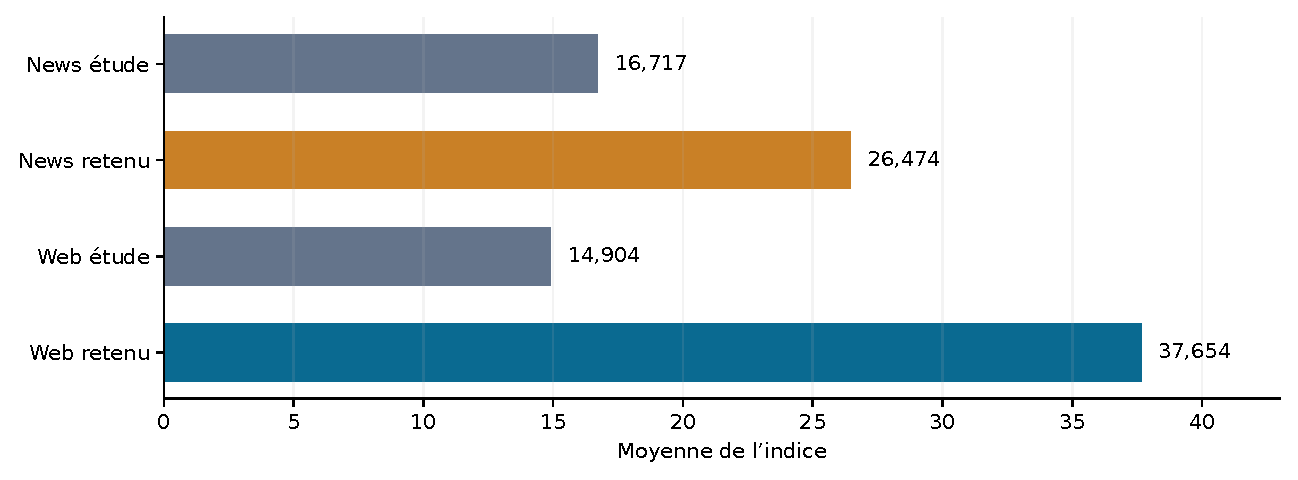
\includegraphics[width=0.9\textwidth]{fig_comparaison.pdf}
\caption{Moyennes des indices : Table 1 de l'article versus données conservées. Il ne s'agit pas d'une comparaison de volumes absolus.}
\end{figure}

\begin{table}[H]
\centering\small
\caption{Quatre observations de \emph{AI News Search} explicitement commentées dans l'article}
\begin{tabular}{@{}lrrr@{}}\toprule
Mois & Article (News) & Notre News & Notre Web\\\midrule
Janvier 2012 & 2 & 4 & 17\\
Mars 2018 & 11 & 32 & 41\\
Novembre 2022 & 16 & 28 & 53\\
Mai 2024 & 86 & 53 & 86\\\bottomrule\end{tabular}
\end{table}

\begin{figure}[H]
\centering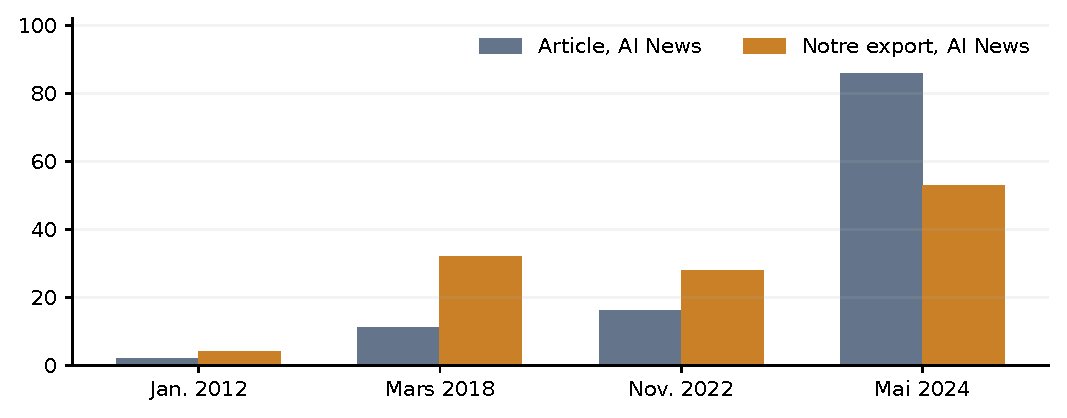
\includegraphics[width=0.86\textwidth]{fig_mois_article.pdf}
\caption{Contrôle des valeurs News de référence : les écarts ne correspondent pas à un simple facteur d'échelle.}
\end{figure}

Le ratio \(GT^{\mathrm{article}}/GT^{\mathrm{reconstitué}}\) des quatre mois News est respectivement \(0{,}500\), \(0{,}344\), \(0{,}571\) et \(1{,}623\). Il n'existe donc \textbf{aucun facteur multiplicatif unique} expliquant ces différences.

Mieux encore, l'ordre de mars 2018 et novembre 2022 est inversé :
\[
 GT^{\mathrm{article}}_{\text{mars 2018}}=11<16=GT^{\mathrm{article}}_{\text{nov. 2022}},
 \qquad
 GT^{\mathrm{équipe}}_{\text{mars 2018}}=32>28=GT^{\mathrm{équipe}}_{\text{nov. 2022}}.
\]
\textbf{Une simple transformation strictement croissante ne peut pas inverser cet ordre.} Notre divergence concerne donc les profils eux-mêmes (requête, mesure historique, échantillonnage ou traitement plus complexe), pas seulement la taille des indices.

\paragraph{La valeur 86 en mai 2024.} L'article l'identifie comme le point haut de son indicateur News, tandis que notre News atteint 100 en juillet 2024. Le fait que notre \emph{Web} soit aussi égal à 86 en mai 2024 est une coïncidence à signaler, non une preuve d'inversion des étiquettes. De plus, un maximum sous 100 sur la période étudiée pourrait provenir d'une fenêtre de normalisation plus large ou d'un traitement non indiqué; ce point n'identifie pas une méthode unique.

\section{Décision de reproduction et protocole opérationnel}
\subsection{Choix définitif}
\keybox{Décision méthodologique}{Les analyses principales utilisent uniquement les deux séries mensuelles fournies : \texttt{Artificial Intelligence}, \textbf{monde entier}, \textbf{toutes catégories}, du 1\textsuperscript{er} janvier 2012 au 31 décembre 2024; propriété Web pour \texttt{AI\_WEB} et propriété News pour \texttt{AI\_NEWS}. Les indices sont conservés \emph{tels quels}, sans centrage-réduction, nouvelle normalisation, interpolation ou moyenne multi-termes.}

\subsection{Conservation, validation et traçabilité}
\begin{enumerate}
\item \textbf{Archiver les CSV bruts :} enregistrer les exports exactement tels qu'ils ont été téléchargés, sans les ouvrir et réenregistrer dans Excel pour préserver le format et les métadonnées textuelles. Dans les noms, distinguer explicitement Web et News.
\item \textbf{Enregistrer les paramètres :} termes, distinction \emph{search term/topic}, dates, région, catégorie, \texttt{gprop}, URL de la requête et date/heure réelle de téléchargement; une date de rédaction du rapport ne saurait remplacer l'horodatage réel de chaque export.
\item \textbf{Contrôler :} 156 dates mensuelles contiguës, unicité de \texttt{DATE}, indices numériques compris entre 0 et 100, absence de cellules manquantes, minima et maxima, rapprochement avec la présente table.
\item \textbf{Produire :} une table \texttt{DATE, AI\_NEWS, AI\_WEB} issue d'une jointure contrôlée sur la date, sans décalage et sans modifier les indices.
\item \textbf{Séparer :} les variantes \texttt{AI}, les comparaisons multi-mots-clés, les fenêtres 2004--2024 et les tests des États-Unis dans un répertoire expérimental, sans confusion avec la base principale.
\item \textbf{Versionner le code et le protocole :} conserver les scripts et notes de décisions dans Git; les CSV bruts peuvent rester hors du dépôt public selon la politique de données de l'équipe.
\end{enumerate}

\begin{table}[H]\centering\small
\caption{Schéma et contrôles de la table de travail}
\begin{tabularx}{\textwidth}{@{}lYY@{}}\toprule
Champ & Définition & Validation\\\midrule
\texttt{DATE} & Date de début du mois (ISO \texttt{YYYY-MM-01}) & 2012-01-01 à 2024-12-01, pas mensuel\\
\texttt{AI\_NEWS} & Indice Google News Search, terme complet & Entier, 0--100, 156 valeurs\\
\texttt{AI\_WEB} & Indice Google Web Search, terme complet & Entier, 0--100, 156 valeurs\\\bottomrule
\end{tabularx}\end{table}

\textbf{Pas de second fichier consolidé.} Le projet utilise déjà le fichier de travail
\texttt{data/processed/ai\_trends\_monthly.csv}, généré par
\texttt{scripts/03\_prepare\_google\_trends.py}. Les deux exports originaux restent
dans \texttt{data/raw/google\_trends/}, séparés par propriété de recherche.
Le présent rapport conserve l'intégralité des 312 indices en annexe, sans introduire de CSV supplémentaire.

\subsection{Utilisation ultérieure dans les modèles de prévision}
Les équations de l'article mobilisent l'indicateur en niveau décalé \(AI_{t-1}\) ainsi que la variation \(\Delta AI_t=AI_t-AI_{t-1}\) \cite{SalisuBadmus2026}. Dans une véritable prévision hors échantillon à l'origine \(t-1\), \textbf{la variation contemporaine \(\Delta AI_t\) n'est pas automatiquement observable}. Il faudra donc expliciter le calendrier de publication, utiliser des variables effectivement disponibles au moment de prévoir, ou qualifier le calcul de maintenant/prévision conditionnelle; sinon, le modèle risque de comporter un biais d'anticipation.

La source Google Trends n'est pas un substitut au contrôle de causalité : une forte association avec les rendements ou la volatilité peut aussi refléter des tendances temporelles communes. La construction des retours, primes de risque et régimes de volatilité fera l'objet d'un traitement distinct.

\section{Critique raisonnée et pistes futures}
\subsection{Ce que l'indicateur mesure, et ce qu'il ne mesure pas}
Un index de recherche agrégée rend compte d'une \emph{attention} pour une expression, non de la portée économique ou de la tonalité des informations. Une rupture technologique majeure, un usage pédagogique et une curiosité générale peuvent tous augmenter l'intérêt de recherche, mais leurs implications pour les cours boursiers peuvent différer. De plus, \texttt{AI} est potentiellement ambigu, alors que \texttt{Artificial Intelligence} est plus spécifique mais linguistiquement plus étroit.

L'existence d'un lien entre attention et marché ne permet pas, sans contrôle, d'isoler l'effet causal d'une nouvelle IA. Les révisions de l'indice, le choix de fenêtre, le type d'interface et l'échantillonnage peuvent affecter les coefficients et les mesures de performance hors échantillon \cite{Cebrian2024,Misuse2025,Liu2024}.

\subsection{Pistes distinctes de la reproduction}
\begin{itemize}
\item \textbf{Sensibilité à la requête :} conserver \texttt{AI} comme série alternative, puis tester explicitement si les conclusions économiques changent de signe ou d'importance statistique.
\item \textbf{Robustesse de millésime :} répéter des téléchargements identiques à des dates différentes, comparer chaque mois, stocker les CSV et métadonnées; ce test n'autorise pas à reconstituer un ancien millésime sans archive réelle.
\item \textbf{Validation externe :} solliciter les CSV originaux et les paramètres complets auprès de l'auteur correspondant. Vérifier aussi la documentation supplémentaire de l'article.
\item \textbf{Extension future, hors réplication :} analyser des articles financiers par des méthodes NLP (thème, sentiment, nouveauté, importance économique), éventuellement via une chaîne d'agents auditables, puis comparer ce signal à Google Trends sans confondre les deux constructions.
\end{itemize}

\subsection{Limites du présent rapport}
La comparaison s'appuie sur les fichiers fournis et les statistiques publiées. \textbf{Nous ne disposons pas des données brutes exactes des auteurs, de leur date de téléchargement ni de leur code complet de collecte.} Nous ne pouvons donc attribuer l'écart à un changement précis de Google Trends, à \texttt{pytrends}, à une erreur des auteurs ou à une opération particulière de transformation. La présente étude documente une non-coïncidence numérique; elle ne démontre pas une faute scientifique.

\section{Conclusion}
Les contrôles montrent que le problème principal ne se situe pas dans notre script de lecture : les téléchargements manuels et \texttt{pytrends} ont fourni des résultats contemporains cohérents. Les expériences portant sur le mot-clé, le pays, la fenêtre et les comparaisons multiples modifient parfois sensiblement les indices, mais ne reproduisent pas de manière justifiée les deux séries publiées. Le contrôle de plusieurs mois exclut en particulier une simple remise à l'échelle monotone de notre variable News.

\textbf{Décision :} préserver les 156 observations Web et les 156 observations News du terme \emph{Artificial Intelligence}, poursuivre les estimations avec une traçabilité explicite, et traiter la divergence comme une limite documentée de la réplication. Les expérimentations alternatives restent disponibles à titre de robustesse, sans remplacement opportuniste des séries retenues.

\clearpage
\section*{Références et sources consultées}
\addcontentsline{toc}{section}{Références et sources consultées}
\begin{thebibliography}{99}\small
\bibitem{SalisuBadmus2026} Salisu, A. A. et Badmus, S. (2026). \emph{Can AI News Improve the Out-of-Sample Forecasts of Risk Premia and Volatility in the U.S. Stock Market?} \emph{Quality \& Quantity}. DOI : \href{https://doi.org/10.1007/s11135-026-02816-9}{10.1007/s11135-026-02816-9}.
\bibitem{GoogleFAQ} Google Trends, \emph{FAQ about Google Trends data}, aide officielle : \url{https://support.google.com/trends/answer/4365533} .
\bibitem{GoogleTerms} Google Trends, \emph{Compare search terms and topics}, aide officielle : \url{https://support.google.com/trends/answer/17309543} .
\bibitem{Cebrian2024} Cebrián, E. et Domenech, J. (2024). \emph{Addressing Google Trends inconsistencies}. \emph{Technological Forecasting and Social Change}, 202, 123318. \url{https://doi.org/10.1016/j.techfore.2024.123318}.
\bibitem{Misuse2025} Hölzl, J., Keusch, F. et Sajons, C. (2025). \emph{The (mis)use of Google Trends data in the social sciences: A systematic review, critique, and recommendations} (2025). \emph{Social Science Research}, 126, 103099. \url{https://pubmed.ncbi.nlm.nih.gov/39909632/}.
\bibitem{Liu2024} Liu, K. (2024). \emph{The measurement errors of google trends data}. \emph{Discover Data}, 2, article 7. \url{https://doi.org/10.1007/s44248-024-00013-3}.
\bibitem{Health2022} \emph{Infodemiologists Beware: Recent Changes to the Google Health Trends API Result in Incomparable Data as of 1 January 2022} (2022). \url{https://pmc.ncbi.nlm.nih.gov/articles/PMC9692853/}.
\bibitem{GoogleAPI2025} Google Search Central (2025). \emph{Google Trends API Alpha}. \url{https://developers.google.com/search/apis/trends}.
\end{thebibliography}

\clearpage
\appendix
\section{Séries mensuelles complètes retenues}\label{annexe_donnees}
\textbf{Source :} deux exports Google Trends portant sur \texttt{Artificial Intelligence}, monde entier, toutes catégories, périodes janvier 2012--décembre 2024; Web et News distinctement configurés. Aucune valeur n'a été corrigée. Les années sont indiquées dans la première ligne de chaque groupe de douze mois.
\small
\setlength{\LTpre}{7pt}
\setlength{\LTpost}{7pt}
\begin{longtable}{@{}lrrr@{}}
\caption{312 observations d'indice, entièrement conservées.}\label{tab:all}\\
\toprule Année & Mois & AI News & AI Web \\\midrule
\endfirsthead
\multicolumn{4}{@{}l}{\footnotesize\color{graytext}\emph{Tableau continué — séries Google Trends retenues}}\\
\toprule Année & Mois & AI News & AI Web \\\midrule
\endhead
\midrule\multicolumn{4}{r}{\footnotesize\itshape Suite sur la page suivante}\\
\endfoot
\bottomrule
\endlastfoot
2012 & 01 & 4 & 17 \\
 & 02 & 5 & 16 \\
 & 03 & 6 & 17 \\
 & 04 & 6 & 14 \\
 & 05 & 6 & 14 \\
 & 06 & 5 & 13 \\
 & 07 & 5 & 13 \\
 & 08 & 4 & 12 \\
 & 09 & 5 & 15 \\
 & 10 & 5 & 16 \\
 & 11 & 20 & 14 \\
 & 12 & 4 & 13 \\
\addlinespace[2pt]
2013 & 01 & 4 & 13 \\
 & 02 & 5 & 14 \\
 & 03 & 4 & 15 \\
 & 04 & 5 & 14 \\
 & 05 & 4 & 14 \\
 & 06 & 4 & 12 \\
 & 07 & 5 & 11 \\
 & 08 & 4 & 12 \\
 & 09 & 4 & 14 \\
 & 10 & 4 & 14 \\
 & 11 & 6 & 14 \\
 & 12 & 6 & 14 \\
\addlinespace[2pt]
2014 & 01 & 5 & 14 \\
 & 02 & 5 & 16 \\
 & 03 & 5 & 14 \\
 & 04 & 6 & 15 \\
 & 05 & 4 & 15 \\
 & 06 & 6 & 13 \\
 & 07 & 6 & 12 \\
 & 08 & 5 & 15 \\
 & 09 & 7 & 15 \\
 & 10 & 7 & 15 \\
 & 11 & 6 & 18 \\
 & 12 & 10 & 17 \\
\addlinespace[2pt]
2015 & 01 & 14 & 17 \\
 & 02 & 21 & 19 \\
 & 03 & 10 & 18 \\
 & 04 & 9 & 18 \\
 & 05 & 29 & 20 \\
 & 06 & 18 & 17 \\
 & 07 & 24 & 19 \\
 & 08 & 13 & 17 \\
 & 09 & 12 & 19 \\
 & 10 & 11 & 19 \\
 & 11 & 13 & 19 \\
 & 12 & 13 & 19 \\
\addlinespace[2pt]
2016 & 01 & 29 & 22 \\
 & 02 & 27 & 20 \\
 & 03 & 21 & 23 \\
 & 04 & 24 & 22 \\
 & 05 & 22 & 22 \\
 & 06 & 25 & 20 \\
 & 07 & 22 & 17 \\
 & 08 & 23 & 17 \\
 & 09 & 41 & 21 \\
 & 10 & 29 & 25 \\
 & 11 & 29 & 26 \\
 & 12 & 35 & 26 \\
\addlinespace[2pt]
2017 & 01 & 33 & 26 \\
 & 02 & 37 & 28 \\
 & 03 & 27 & 30 \\
 & 04 & 24 & 29 \\
 & 05 & 23 & 31 \\
 & 06 & 25 & 27 \\
 & 07 & 24 & 29 \\
 & 08 & 31 & 33 \\
 & 09 & 29 & 38 \\
 & 10 & 33 & 41 \\
 & 11 & 32 & 46 \\
 & 12 & 33 & 40 \\
\addlinespace[2pt]
2018 & 01 & 29 & 49 \\
 & 02 & 32 & 44 \\
 & 03 & 32 & 41 \\
 & 04 & 33 & 40 \\
 & 05 & 33 & 42 \\
 & 06 & 36 & 37 \\
 & 07 & 28 & 36 \\
 & 08 & 32 & 35 \\
 & 09 & 31 & 40 \\
 & 10 & 34 & 41 \\
 & 11 & 36 & 41 \\
 & 12 & 32 & 39 \\
\addlinespace[2pt]
2019 & 01 & 31 & 42 \\
 & 02 & 35 & 42 \\
 & 03 & 34 & 42 \\
 & 04 & 33 & 42 \\
 & 05 & 32 & 44 \\
 & 06 & 29 & 42 \\
 & 07 & 34 & 41 \\
 & 08 & 33 & 39 \\
 & 09 & 30 & 46 \\
 & 10 & 32 & 43 \\
 & 11 & 34 & 49 \\
 & 12 & 32 & 39 \\
\addlinespace[2pt]
2020 & 01 & 33 & 43 \\
 & 02 & 33 & 47 \\
 & 03 & 16 & 39 \\
 & 04 & 19 & 39 \\
 & 05 & 20 & 39 \\
 & 06 & 21 & 37 \\
 & 07 & 20 & 36 \\
 & 08 & 20 & 38 \\
 & 09 & 22 & 41 \\
 & 10 & 22 & 40 \\
 & 11 & 22 & 38 \\
 & 12 & 18 & 39 \\
\addlinespace[2pt]
2021 & 01 & 19 & 37 \\
 & 02 & 21 & 41 \\
 & 03 & 18 & 38 \\
 & 04 & 21 & 38 \\
 & 05 & 18 & 38 \\
 & 06 & 18 & 40 \\
 & 07 & 16 & 38 \\
 & 08 & 17 & 39 \\
 & 09 & 22 & 41 \\
 & 10 & 27 & 41 \\
 & 11 & 27 & 43 \\
 & 12 & 29 & 38 \\
\addlinespace[2pt]
2022 & 01 & 23 & 46 \\
 & 02 & 24 & 53 \\
 & 03 & 23 & 51 \\
 & 04 & 28 & 53 \\
 & 05 & 26 & 50 \\
 & 06 & 26 & 55 \\
 & 07 & 25 & 48 \\
 & 08 & 27 & 49 \\
 & 09 & 27 & 54 \\
 & 10 & 27 & 51 \\
 & 11 & 28 & 53 \\
 & 12 & 36 & 56 \\
\addlinespace[2pt]
2023 & 01 & 37 & 64 \\
 & 02 & 37 & 74 \\
 & 03 & 42 & 75 \\
 & 04 & 47 & 81 \\
 & 05 & 58 & 100 \\
 & 06 & 54 & 89 \\
 & 07 & 58 & 83 \\
 & 08 & 48 & 76 \\
 & 09 & 50 & 76 \\
 & 10 & 47 & 79 \\
 & 11 & 53 & 79 \\
 & 12 & 46 & 73 \\
\addlinespace[2pt]
2024 & 01 & 49 & 81 \\
 & 02 & 60 & 85 \\
 & 03 & 56 & 80 \\
 & 04 & 56 & 81 \\
 & 05 & 53 & 86 \\
 & 06 & 84 & 84 \\
 & 07 & 100 & 75 \\
 & 08 & 97 & 77 \\
 & 09 & 92 & 83 \\
 & 10 & 82 & 80 \\
 & 11 & 78 & 78 \\
 & 12 & 63 & 78 \\
\addlinespace[2pt]

\end{longtable}
\normalsize

\section{Annexe de provenance informatique}
\begin{table}[H]\centering\small
\caption{Repères permettant de reconstruire la collecte}
\begin{tabularx}{\textwidth}{@{}p{3.4cm}Y@{}}\toprule
Élément & Repère\\\midrule
Exploration Web & \url{https://trends.google.com/trends/explore} -- termes, période et propriété Web indiqués dans le tableau 1\\
Exploration News & \url{https://trends.google.com/trends/explore} -- mêmes paramètres, propriété \texttt{gprop=news}\\
Fichier de travail existant & \texttt{data/processed/ai\_trends\_monthly.csv}\\
Colonnes & \texttt{DATE}, \texttt{AI\_NEWS}, \texttt{AI\_WEB}\\
Calcul des statistiques & Moyenne arithmétique; écart-type empirique avec correction \(n-1\)\\
Export brut & Entête Google Trends «\,Catégorie : Toutes catégories\,» et «\,Mois,Artificial Intelligence: (Dans tous les pays)\,»\\\bottomrule
\end{tabularx}
\end{table}
\paragraph{Note finale.} Le type de recherche (Web ou News) est établi par le paramétrage vérifié et son URL, non par l'en-tête du CSV, qui ne transporte pas \texttt{gprop}. Pour assurer la répétabilité, il faut conserver les deux URL en même temps que les fichiers bruts et les dates de collecte.
\end{document}
